\section{tf.estimator快速导航}
TensorFlow的高级机器学习API(tf.estimator)使得配置,训练评价多种机器学习模型变得很简单,在这个导航中,你讲用tf.estimator构造一个神经网络分类器在\href{https://en.wikipedia.org/wiki/Iris_flower_data_set}{iris data}基于花萼和花瓣的几何特性训练预测花的种类,你的代码按照如下5步执行:
\begin{enumerate}
	\item 载入CSV文件的训练测试数据到TensorFlowDataset
	\item 构造\href{https://www.tensorflow.org/api_docs/python/tf/estimator/DNNClassifier}{神经网络分类器}
	\item 用训练数据训练模型。
	\item 评估模型的精度。
	\item 分类新的样本
\end{enumerate}
\subsection{完成神经网络源代码}
\begin{python}
from __future__ import absolute_import
from __future__ import division
from __future__ import print_function

import os
import urllib

import numpy as np
import tensorflow as tf

# Data sets
IRIS_TRAINING = "iris_training.csv"
IRIS_TRAINING_URL = "http://download.tensorflow.org/data/iris_training.csv"

IRIS_TEST = "iris_test.csv"
IRIS_TEST_URL = "http://download.tensorflow.org/data/iris_test.csv"

def main():
  # If the training and test sets aren't stored locally, download them.
  if not os.path.exists(IRIS_TRAINING):
    raw = urllib.urlopen(IRIS_TRAINING_URL).read()
    with open(IRIS_TRAINING, "w") as f:
      f.write(raw)

  if not os.path.exists(IRIS_TEST):
    raw = urllib.urlopen(IRIS_TEST_URL).read()
    with open(IRIS_TEST, "w") as f:
      f.write(raw)

  # Load datasets.
  training_set = tf.contrib.learn.datasets.base.load_csv_with_header(
      filename=IRIS_TRAINING,
      target_dtype=np.int,
      features_dtype=np.float32)
  test_set = tf.contrib.learn.datasets.base.load_csv_with_header(
      filename=IRIS_TEST,
      target_dtype=np.int,
      features_dtype=np.float32)

  # Specify that all features have real-value data
  feature_columns = [tf.feature_column.numeric_column("x", shape=[4])]

  # Build 3 layer DNN with 10, 20, 10 units respectively.
  classifier = tf.estimator.DNNClassifier(feature_columns=feature_columns,
                                          hidden_units=[10, 20, 10],
                                          n_classes=3,
                                          model_dir="/tmp/iris_model")
  # Define the training inputs
  train_input_fn = tf.estimator.inputs.numpy_input_fn(
      x={"x": np.array(training_set.data)},
      y=np.array(training_set.target),
      num_epochs=None,
      shuffle=True)

  # Train model.
  classifier.train(input_fn=train_input_fn, steps=2000)

  # Define the test inputs
  test_input_fn = tf.estimator.inputs.numpy_input_fn(
      x={"x": np.array(test_set.data)},
      y=np.array(test_set.target),
      num_epochs=1,
      shuffle=False)

  # Evaluate accuracy.
  accuracy_score = classifier.evaluate(input_fn=test_input_fn)["accuracy"]

  print("\nTest Accuracy: {0:f}\n".format(accuracy_score))

  # Classify two new flower samples.
  new_samples = np.array(
      [[6.4, 3.2, 4.5, 1.5],
       [5.8, 3.1, 5.0, 1.7]], dtype=np.float32)
  predict_input_fn = tf.estimator.inputs.numpy_input_fn(
      x={"x": new_samples},
      num_epochs=1,
      shuffle=False)

  predictions = list(classifier.predict(input_fn=predict_input_fn))
  predicted_classes = [p["classes"] for p in predictions]

  print(
      "New Samples, Class Predictions:    {}\n"
      .format(predicted_classes))

if __name__ == "__main__":
    main()
\end{python}
下面的章节将详细介绍代码。
\subsection{载入CSV数据进入TensorFlow}
\href{https://en.wikipedia.org/wiki/Iris_flower_data_set}{Iris data set}包含有150行iris瓶中的样本:Iris setosa, Iris virginica和Iris versicolor。
\begin{figure}[h]
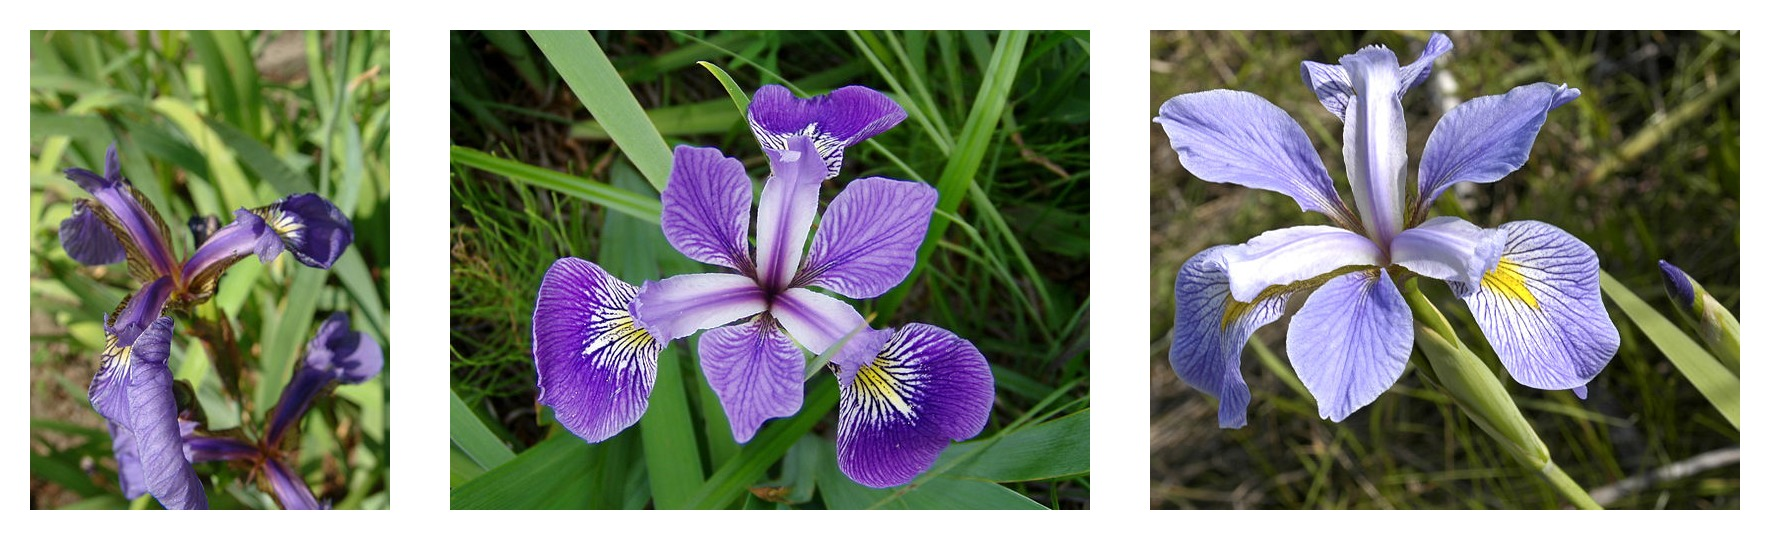
\includegraphics[scale=0.6]{iris_three_species}
\end{figure}
每行的数据包括花萼的长宽,花瓣的长宽,花用整数代表0表示Iris setosa,1表示 Iris versicolor,2表示Iris virginica。
iris数据集已经被分成两部分
\begin{itemize}
	\item 120个样本的训练集\href{http://download.tensorflow.org/data/iris_training.csv}{iris_training.csv}
	\item 30个样本的测试集\href{http://download.tensorflow.org/data/iris_test.csv}{iris_test.csv}
\end{itemize}
导入需要的模型
\begin{python}
from __future__ import absolute_import
from __future__ import division
from __future__ import print_function

import os
import urllib

import tensorflow as tf
import numpy as np

IRIS_TRAINING = "iris_training.csv"
IRIS_TRAINING_URL = "http://download.tensorflow.org/data/iris_training.csv"

IRIS_TEST = "iris_test.csv"
IRIS_TEST_URL = "http://download.tensorflow.org/data/iris_test.csv"
\end{python}
如果训练集和测试集没有被存储在本地,下载他们:
\begin{python}
if not os.path.exists(IRIS_TRAINING):
  raw = urllib.urlopen(IRIS_TRAINING_URL).read()
  with open(IRIS_TRAINING,'w') as f:
    f.write(raw)

if not os.path.exists(IRIS_TEST):
  raw = urllib.urlopen(IRIS_TEST_URL).read()
  with open(IRIS_TEST,'w') as f:
    f.write(raw)
\end{python}
下一步用learn.dataset.base中的load\_csv\_with\_header()方法载入训练数据进入Dataset,load\_csv\_with\_header()方法接受三个参数:
\begin{itemize}
	\item filename:CSV文件的完成的路径加上文件名。
	\item target\_dtype:接收numpy datatype的数据集的目标值。
	\item feature\_dtype:接收numpy datatype类型的数据集的特征值。
\end{itemize}
这里的目标(你的训练模型的预测)是花的种类,值范围为0~2,因此合适的numpy数据类型是np.int。
\begin{python}
# Load datasets.
training_set = tf.contrib.learn.datasets.base.load_csv_with_header(
    filename=IRIS_TRAINING,
    target_dtype=np.int,
    features_dtype=np.float32)
test_set = tf.contrib.learn.datasets.base.load_csv_with_header(
    filename=IRIS_TEST,
    target_dtype=np.int,
    features_dtype=np.float32)
\end{python}
在tf.contrib.learn中的Dataset是\href{https://docs.python.org/2/library/collections.html#collections.namedtuple}{named tuples};你可以通过data和target访问特征数据和目标值,这里training\_set和training\_set.target包含训练集的特征数据和目标数据,对应的test\_set.data和test\_set.target包含测试集特征和目标。
\subsection{构造神经网络分类器}
tf.estimator提供多种预定义方法,称为Estimator,你可以在同国内你的数据"盒,子"运行训练,评估操作,你可以实例化tf.estimator.DNNClassfier:
\begin{python}
# Specify that all features have real-value data
feature_columns = [tf.feature_column.numeric_column("x", shape=[4])]

# Build 3 layer DNN with 10, 20, 10 units respectively.
classifier = tf.estimator.DNNClassifier(feature_columns=feature_columns,
                                        hidden_units=[10, 20, 10],
                                        n_classes=3,
                                        model_dir="/tmp/iris_model")
\end{python}
下面的代码中首先定义模型的特征列,指定在数据集中的特征的数据类型。所有的特征数据是连续的,因此tf.feature\_column.number\_column是构造特征列的合适的函数,数据集中有4个特征,因此我们指定shape为[4]保持所有的数据,然后用下面的参数创建DNNClassfier分类器模型:
\begin{itemize}
	\item feature_columns=feature_columns,特征集合的列。
	\item hidden\_units=[10,20,10],三个\href{http://stats.stackexchange.com/questions/181/how-to-choose-the-number-of-hidden-layers-and-nodes-in-a-feedforward-neural-netw}{hidden layer}包含有10,,2,10个神经元。
	\item n\_classes=3,三个目标类,对应三个iris种类。
	\item model\_dir=/temp/iris\_model:训练模型中保存checkpoint文件的路径
\end{itemize}
\subsection{描述训练的输入pipline}
tf.estimator API用输入函数创建TensorFlow操作为模型生成数据,你可以用tf.estimator.numpy\_input\-fn生成输入pipeline:
\begin{python}
# Define the training inputs
train_input_fn = tf.estimator.inputs.numpy_input_fn(
    x={"x": np.array(training_set.data)},
    y=np.array(training_set.target),
    num_epochs=None,
    shuffle=True)
\end{python}
\subsection{为iris训练集拟合DNNClassfier}
现在我们已经配置好的classfier模型,你可以用train方法通过训练数据训练模型。传递train\_input\_fn作为input\_fn,这里训练步数为2000:
\begin{python}
# Train model.
classifier.train(input_fn=train_input_fn, steps=2000)
\end{python}
状态模型每保存在classfier,依偎着你可以反复训练,例如下面是合适的:
\begin{python}
classifier.train(input_fn=train_input_fn, steps=1000)
classifier.train(input_fn=train_input_fn, steps=1000)
\end{python}
然而,如果你在训练的时候跟踪模型,你可以用TensorFlow \href{https://www.tensorflow.org/api_docs/python/tf/train/SessionRunHook}{SessionRunHook}执行采集操作.
\subsection{评估模型的精度}
你可以在Iris训练集上训练你的DNNClassfier模型;现在你可以在测试集上用evaluate检查它在测试集上个精确度。evaluate返回一个评估结果的字典,下面的代码春娣Irish测数据给test\_set.data和test\_set.target评估和从结果中打印。
\begin{python}
# Define the test inputs
test_input_fn = tf.estimator.inputs.numpy_input_fn(
    x={"x": np.array(test_set.data)},
    y=np.array(test_set.target),
    num_epochs=1,
    shuffle=False)

# Evaluate accuracy.
accuracy_score = classifier.evaluate(input_fn=test_input_fn)["accuracy"]

print("\nTest Accuracy: {0:f}\n".format(accuracy_score))
\end{python}
\begin{quote}
\emph{这里num\_epochs=1参数对于numpy\_input\_fn是很重要的。test\_input\_fn将在数据上迭代一次然后报出OutOfRangeError,这个错误通知分类及停止评估,因此它将计算输入一次}
\end{quote}
然后你可以运行完整的脚本,它将打印出:
\begin{python}
Test Accuracy: 0.966667
\end{python}
你的精度结果可能有点不同但是应该大于90\%。
\subsection{分类新的样本}
用estimator的predict()方法分类新的样本,例如你有两个新的花的样本:
\begin{tabular}{|c|c|c|c|}
花萼长度&花萼宽度&花瓣长度&花瓣宽度\\
6.4&3.2&4.5&1.5\\
5.8&3.1&5.0&1.7\\
\end{tabular}
你可以用predict(方法预测结果,predict返回一个词典生成器,生成器可以容易的被转化成列表,下面的代码访问和打印预测的类:
\begin{python}
# Classify two new flower samples.
new_samples = np.array(
    [[6.4, 3.2, 4.5, 1.5],
     [5.8, 3.1, 5.0, 1.7]], dtype=np.float32)
predict_input_fn = tf.estimator.inputs.numpy_input_fn(
    x={"x": new_samples},
    num_epochs=1,
    shuffle=False)

predictions = list(classifier.predict(input_fn=predict_input_fn))
predicted_classes = [p["classes"] for p in predictions]

print(
    "New Samples, Class Predictions:    {}\n"
    .format(predicted_classes))
\end{python}
你应该得到如下结果
\begin{python}
New Samples, Class Predictions:    [1 2]
\end{python}
结果预测样本是 Iris versicolor, Iris virginica。
\section{用tf.estimator创建一个输入函数}
在这个导航中向你介绍在tf.estimator创建一个输入函数。你将看到如何构造一个input\_fn去处理和输入数据进你的模型,然后模拟将实现一个input\_函数到神经网络回归器训练,评估预测房价数据
\subsection{用input\_fn自定义Pipeline}
input\_n被用来传递特征和目标数据到Estimator的train,evaluate,predict方法。
\begin{python}
import numpy as np

training_set = tf.contrib.learn.datasets.base.load_csv_with_header(
    filename=IRIS_TRAINING, target_dtype=np.int, features_dtype=np.float32)

train_input_fn = tf.estimator.inputs.numpy_input_fn(
    x={"x": np.array(training_set.data)},
    y=np.array(training_set.target),
    num_epochs=None,
    shuffle=True)

classifier.train(input_fn=train_input_fn, steps=2000)
\end{python}
\subsection{input\_fn的分解}
下面的代码描述了输入函数的基本结构:
\begin{python}
def my_input_fn():

    # Preprocess your data here...

    # ...then return 1) a mapping of feature columns to Tensors with
    # the corresponding feature data, and 2) a Tensor containing labels
    return feature_cols, labels
\end{python}
输入函数的函数体包含指定处理你的输入数据的逻辑,像数据清洗和\href{https://en.wikipedia.org/wiki/Feature_scaling}{特征放大},输入函数必须返回两个包含最终的标签和特征的数据输入进你的模型:

featrue\_cols:一个包含有映射特征列名字为Tensor包含有特征数据的键值(key/value)对。

labels:一个包含有你的标签的值(你的模型想要预测的值)
\subsection{转换特征数据为Tensor}
如果你的feature/label数据是一个python数据,或者pandas dateframe或者numpy数组,你可以用下面的方法构造
input\_fn:
\begin{python}
import numpy as np
# numpy input_fn.
my_input_fn = tf.estimator.inputs.numpy_input_fn(
    x={"x": np.array(x_data)},
    y=np.array(y_data),
    ...)
\end{python}
\begin{python}
import pandas as pd
# pandas input_fn.
my_input_fn = tf.estimator.inputs.pandas_input_fn(
    x=pd.DataFrame({"x": x_data}),
    y=pd.Series(y_data),
    ...)
\end{python}
对于\href{https://en.wikipedia.org/wiki/Sparse_matrix}{稀疏,分类数据},你将需要填入下面三个参数:
\begin{itemize}
	\item dense\_shape:形状tensor。每个维度的列表的索引。例如dense\_shape=[3,6]指定二维tensor,$3\times6$,dense\_shape=[2,3,4]指定3维$2\times3\times4$tensor,dense\_shape=[9]指定包含9个元素的一维tensor。
	\item indices:在你的包含有非零值的tensor的元素的索引。接受列表,列表中的每个元素是包含非0元素的索引。(例如[0,0]代表两维Tensor的第0行第0列。indices=[[1,3],[2,4]]指定索引为[1,3],[2,4]的元素有非零值。)
	\item values:一维值得tensor,values中的i对应indices中的i和它指定的值。例如给定值indices=[[1,3],[2,4]],参数values=[18,3.6],指定元素索引[1,3]的位置为18,[2,4]的值为3.6。
\end{itemize}
下面的代码顶一个一个两维$3\times5$的SparseTensor,索引为[0,1]的位置的值为6,[2,4]位置的值为0.5,其他值为0。
\begin{python}
sparse_tensor = tf.SparseTensor(indices=[[0,1], [2,4]],
                                values=[6, 0.5],
                                dense_shape=[3, 5])
\end{python}
对应的tensor:
\begin{python}
[[0, 6, 0, 0, 0]
 [0, 0, 0, 0, 0]
 [0, 0, 0, 0, 0.5]]
\end{python}
\subsection{传递input\_fn数据到你的模型}
为了输入数据给你的模型训练,你简单的传递你创建的输入函数给你的train操作:
\begin{python}
classifier.train(input_fn=my_input_fn, steps=2000)
\end{python}
注意input\_fn参数必须接受一个函数对象(例如input\_fn=input\_fn),这意味着如果你在训练调用的时候传递参数给你的input\_fn,不是函数调用的返回值,正如下面的代码一样,你将得到TypeError:
\begin{python}
classifier.train(input_fn=my_input_fn(training_set), steps=2000)
\end{python}
然而如果你想参数化你的输入函数,有其它的方法能做到,你可以实现一个包装器函数不接受参数input\_fn用它实现你想要的参数输入函数。
\begin{python}
def my_input_fn(data_set):
  ...

def my_input_fn_training_set():
  return my_input_fn(training_set)

classifier.train(input_fn=my_input_fn_training_set, steps=2000)
\end{python}
你同样可以用Python的\href{https://docs.python.org/2/library/functools.html#functools.partial}{function.pattial}函数构造一个新的参数固定的函数对象。
\begin{python}
classifier.train(
    input_fn=functools.partial(my_input_fn, data_set=training_set),
    steps=2000)
\end{python}
第三个选择是用lambda表达式包装你的input\_fn函数传递它给你的input\_fn参数:
\begin{python}
classifier.train(input_fn=lambda: my_input_fn(training_set), steps=2000)
\end{python}
用上面的方法的一个很大的好处是为你的数据集接受参数,你可以通过改变数据集参数传递相同的input\_fn函数给evaluate和prediction操作:
\begin{python}
classifier.evaluate(input_fn=lambda: my_input_fn(test_set), steps=2000)
\end{python}
这种方法加强的代码的维护性:不需要定义多的input\_fn函数(例如input\_fn\_train,input\_fn\_test,input\_fn\_prediction)给每个操作,最终你可以用tf.estimator.inputs中的方法从numpy或者pandas数据集创建input\_fn。另一个好处是你可以用更多的参数,像num\_epochs和shuffle控制input\_fn如何在数据上迭代,
\begin{python}
import pandas as pd

def get_input_fn_from_pandas(data_set, num_epochs=None, shuffle=True):
  return tf.estimator.inputs.pandas_input_fn(
      x=pdDataFrame(...),
      y=pd.Series(...),
      num_epochs=num_epochs,
      shuffle=shuffle)
\end{python}
\begin{python}
import numpy as np

def get_input_fn_from_numpy(data_set, num_epochs=None, shuffle=True):
  return tf.estimator.inputs.numpy_input_fn(
      x={...},
      y=np.array(...),
      num_epochs=num_epochs,
      shuffle=shuffle)
\end{python}
\subsection{波士顿房价的神经网络模型}
接下来的导航,你将写输入函数处理从\href{https://archive.ics.uci.edu/ml/datasets/Housing}{UCI Gousing Data Set}获取的数据集的子集,传递数据给神经网络回归器预测房价
你讲用于训练的神经网络包含下面的子集\href{https://www.tensorflow.org/get_started/input_fn#setup}{Boston CSV data sets}包含下面\href{https://archive.ics.uci.edu/ml/machine-learning-databases/housing/housing.names}{特征数据}
\begin{tabular}{|c|c|}
\hline
特征&描述\\
CRIM&人均犯罪率\\
ZN&居住地面积划分为25000平方英尺一块\\
INDUS&非商业用地的一部分\\
NOX&一氧化氮的浓度为千万分之一\\
RM&每个房子的房间数\\
AGE&1940年前自有居民的比例\\
DIS&离波士顿就业中心的距离\\
TAX&每10000美元的税率\\
PTRATIO&学生老师的比率
\end{tabular}
\subsection{建立}
下载数据集\href{http://download.tensorflow.org/data/boston_train.csv}{boston_train.csv},\href{http://download.tensorflow.org/data/boston_test.csv}{boston_test.csv}和\href{http://download.tensorflow.org/data/boston_predict.csv}{boston_predict.csv}
\subsection{导入的房子数据}
\begin{python}
from __future__ import absolute_import
from __future__ import division
from __future__ import print_function

import itertools

import pandas as pd
import tensorflow as tf

tf.logging.set_verbosity(tf.logging.INFO)
\end{python}
给CULUMNS中的数据定义名字,区别于标签中的特征,定义FEATURES和LABEL,读入CSV文件到pandas DataFrame:
\begin{python}
COLUMNS = ["crim", "zn", "indus", "nox", "rm", "age",
           "dis", "tax", "ptratio", "medv"]
FEATURES = ["crim", "zn", "indus", "nox", "rm",
            "age", "dis", "tax", "ptratio"]
LABEL = "medv"

training_set = pd.read_csv("boston_train.csv", skipinitialspace=True,
                           skiprows=1, names=COLUMNS)
test_set = pd.read_csv("boston_test.csv", skipinitialspace=True,
                       skiprows=1, names=COLUMNS)
prediction_set = pd.read_csv("boston_predict.csv", skipinitialspace=True,
                             skiprows=1, names=COLUMNS)
\end{python}
\subsection{定义特征列创建回归器}
下一步是为输入数据创建FeatureColumn,数据的格式指定用于训练的特征集,因为所有在房价数据集中的的特征包含连续的值,你可以用tf.contrib.layers.real\_valued\_column()创建他们的FeatureColumn:
\begin{python}
feature_cols = [tf.feature_column.numeric_column(k) for k in FEATURES]
\end{python}
现在初始化一个神经网络回归模型的实体DNNRegressor,你需要提供两个参数:hidden\_units指定每个隐藏层的节点数(这里的两层,每层10个节点)和feature\_columns:包含FeatureColumns
\begin{python}
regressor = tf.estimator.DNNRegressor(feature_columns=feature_cols,
                                      hidden_units=[10, 10],
                                      model_dir="/tmp/boston_model")
\end{python}
\subsection{构建input\_fn}
传递输入数据给regressor,写一个factory方法接受pandas DataFrame返回一个input\_fn:
\begin{python}
def get_input_fn(data_set, num_epochs=None, shuffle=True):
  return tf.estimator.inputs.pandas_input_fn(
      x=pd.DataFrame({k: data_set[k].values for k in FEATURES}),
      y = pd.Series(data_set[LABEL].values),
      num_epochs=num_epochs,
      shuffle=shuffle)
\end{python}
注意输入数据被传递给input\_fn的data\_set参数,这意味着函数可以处理任何你导入的的DataFrame:training\_set,test\_set和prediction\_set。提供两个额外的参数num\_epochs(控制在数据上的迭代次数)训练的时候设置为None,因此input\_fn保持返回值知道训练步数到达,为了平局和测试设置为1,因此input\_fn将在数据上迭代然后抛出OutOfRangeError,错误将通知Estimator停止评估或者预测:shuffle(是否打乱数据)。对于评估和预测,设置为False,因此input\_fn在数据上顺序迭代,对于训练设置为True。
\subsection{训练回归器}
为了训练神经网络回归器,用training\_set传递给input\_fn运行train:
\begin{python}
regressor.train(input_fn=get_input_fn(training_set), steps=5000
\end{python}
你应该能看到类似的输出,每100步报告训练的损失:
\begin{python}
INFO:tensorflow:Step 1: loss = 483.179
INFO:tensorflow:Step 101: loss = 81.2072
INFO:tensorflow:Step 201: loss = 72.4354
...
INFO:tensorflow:Step 1801: loss = 33.4454
INFO:tensorflow:Step 1901: loss = 32.3397
INFO:tensorflow:Step 2001: loss = 32.0053
INFO:tensorflow:Step 4801: loss = 27.2791
INFO:tensorflow:Step 4901: loss = 27.2251
INFO:tensorflow:Saving checkpoints for 5000 into /tmp/boston_model/model.ckpt.
INFO:tensorflow:Loss for final step: 27.1674.
\end{python}
\subsection{评估模型}
下一步看看模型在测试数据及上的性能,运行evaluate,传递test\_set到input\_fn:
\begin{python}
ev = regressor.evaluate(
    input_fn=get_input_fn(test_set, num_epochs=1, shuffle=False))
\end{python}
从ev结果返回损失的,打印:
\begin{python}
loss_score = ev["loss"]
print("Loss: {0:f}".format(loss_score))
\end{python}
你应该能看到下面的结果:
\begin{python}
INFO:tensorflow:Eval steps [0,1) for training step 5000.
INFO:tensorflow:Saving evaluation summary for 5000 step: loss = 11.9221
Loss: 11.92209
\end{python}
\subsection{做出预测}
最后你可以用模型在给定的预测包含特征数据没有标签的数据集上预测房价
\begin{python}
y = regressor.predict(
    input_fn=get_input_fn(prediction_set, num_epochs=1, shuffle=False))
# .predict() returns an iterator of dicts; convert to a list and print
# predictions
predictions = list(p["predictions"] for p in itertools.islice(y, 6))
print("Predictions: {}".format(str(predictions))
\end{python}
你应该得到包含6个房价值(单位是千美元)
\begin{python}
Predictions: [ 33.30348587  17.04452896  22.56370163  34.74345398  14.55953979
  19.58005714]
\end{python}